\documentclass[10pt,letterpaper,twoside,twocolumn]{article}   %tipo de doc
%------------------ PAQUETES PRINCIPALES ------------------------------
\usepackage[T1]{fontenc}                          %especificando fuente
\usepackage[utf8]{inputenc}                       %codificacion
\usepackage[spanish,english]{babel}               %idioma del documento
\usepackage{scrbase}                              %paquete KOMA-script 
\usepackage{caption}                              %modificacion del caption para imagenes y tablas
\DeclareCaptionLabelSeparator{point}{. }
\captionsetup{labelsep=point}
\usepackage{pdfpages}                             %agregar header en pdf
\usepackage{amsmath}                              %ec.matematicas
\usepackage{amsfonts}                             %ec.matematicas
\usepackage{amssymb}                              %ec.matematicas
\usepackage{mathtext}                             %caracteres especiales ec. matem.
\usepackage{amsthm}                               %paquete matematico
\usepackage{makeidx}                              %gen. de indices
\usepackage{graphicx}                             %insertar imagenes
\usepackage{epsfig}                               %insertar imagenes
\usepackage{lmodern}                              %fuente del doc
\usepackage{kpfonts}                              %fuente del doc
\usepackage{bm}                                   %negrita en ec.
\usepackage{booktabs}                             %paquete de tablas
\usepackage{tabularx}                             %paquete de tablas
\usepackage{dcolumn}                              %paquete de tablas
\usepackage{latexsym}                             %paquete de simbolos
\usepackage{algorithm}                            %paquete para escribir algoritmos
\usepackage{fancyhdr}                             %Fancy Header / Footer (encabezado y pie de pag)
\usepackage{ragged2e}                             %justificado del texto
\usepackage{titlesec}                             %para modificar el formato del titulos
\usepackage{url}                                  %URL en bibliografia
\usepackage{dirtytalk}                            %Easy quotes
\usepackage[shortlabels]{enumitem}
\usepackage[left=2.5cm,right=2.5cm,top=2.5cm,bottom=2.5cm]{geometry}
\setlength{\parindent}{0cm}                       %quitar sangría
\raggedbottom
%-------------------PIE DE PAG Y OTROS DEL DOCUMENTO (NO MODIFICAR) ------------
% usado el \thispagestyle para la primera pag y \pagestyle para las demas
\fancyhf{}
\renewcommand{\headrulewidth}{0pt}
\renewcommand{\footrulewidth}{0pt}
\pagestyle{fancy}
\lhead[\vspace{1ex}\thepage]{{\vspace{1ex} \footnotesize El estado de la metodología de sistemas blandos en los últimos 10 años.}}
\chead[]{}
\rhead[\vspace{1ex} \footnotesize{D. Delgado, L. Hernández}]{\raisebox{-0.5\height}{
\includegraphics[scale=0.15]{LogoUIS_Ingenierias.jpg}}\qquad {\thepage} }
\lfoot[]{}
\cfoot[]{}
\rfoot[]{}
\fancypagestyle{Primera_Pagina}{
\lfoot{ISSN Printed: 1657 - 4583, ISSN Online: 2145 – 8456, CC BY-ND 4.0}
\cfoot[]{}
\rfoot[]{}
}
%-------------------- DOCUMENTO -----------------------------
\begin{document}
\selectlanguage{spanish}
%------------ COMANDOS DE ARTICULO (NO MODIFICAR) ---------------------------
\thispagestyle{Primera_Pagina}
\newcommand{\titulos}[2]{
\begin{center}
\vspace{4ex}
{\LARGE \textbf{#1}}\\
\hrulefill \\
\vspace{1ex}
{\LARGE \textbf{#2}}
\end{center}
}
\newcommand{\autores}[1]{
\vspace{1ex}\begin{center}
\textbf{#1}
\end{center}
}
\newcommand{\infoautores}[1]{
\vspace{0ex}\begin{center}
#1
\end{center}
}
\newcommand{\resumenESP}[1]{\textbf{Resumen:}\\
\\
#1\\
\\}
\newcommand{\resumenING}[1]{\textbf{Abstract:}\\
\\
#1\\
\\}
\newcommand{\palabrasESP}[1]{\textbf{Palabras clave:} #1\\
\\}
\newcommand{\palabrasING}[1]{\textbf{Keywords:} #1\\
\\}
\newcommand{\fechas}[3]{
\begin{center}
Recibido: #1. Aceptado: #2. Versión final: #3.\\
\end{center} 
}
\newcommand{\encabezadoUIS}{
\begin{center}
 
\includepdf[pages={1}]{HeaderUIS_Ingenierias.pdf}
\end{center}
}
% modificacion de los labels para los titutlos y subtitulos
%\titleformat{comando}{formato}{formato del texto}{formato del label}{separacion}{antes}{dps}
\titleformat{\section}[block]{\normalsize\bfseries}{\normalsize\bfseries\thesection}{0.1cm}{}{}
\titleformat{\subsection}[block]{\normalsize\bfseries}{\normalsize\bfseries\thesubsection}{0.1cm}{}{}
\titleformat{\subsubsection}[block]{\normalsize\bfseries}{\normalsize\bfseries\thesubsubsection}{0.1cm}{}{}
% modificacion de los labels para las tablas y figuras
%\renewcaptionname{idioma}{\comando}{nombre nuevo}
\renewcaptionname{english}{\figurename}{Figure}
\renewcaptionname{english}{\tablename}{Table}
\renewcaptionname{spanish}{\figurename}{Figura}
\renewcaptionname{spanish}{\tablename}{Tabla}
%------------------INGRESE TITULOS Y RESUMENES ----------------
\twocolumn[{
\thispagestyle{Primera_Pagina}
\encabezadoUIS % no modificar
\titulos{El estado de la metodología de sistemas blandos en los últimos 10 años.}{The state of soft systems methodology in the last 10 years.}
\autores{Daniel David Delgado Cervantes$^{1}$, Laura Alexandra Hernández Pérez$^{2}$} 
\infoautores{
$^{1}$Escuela de Ingeniería de Sistemas, Universidad Industrial de Santander. Correo electrónico: daniel2182066@correo.uis.edu.co\\
$^{2}$Escuela de Ingeniería de Sistemas, Universidad Industrial de Santander. Correo electrónico: laura2182054@correo.uis.edu.co\\
}

\resumenESP{En el presente artículo, se efectuó una revisión bibliográfica de la metodología de sistemas blandos (MSB) ha tenido en la última década. Esto se realizó con el fin de entender el estado en el que se encuentra la MSB en términos de popularidad al igual que el entendimiento de los campos en los cuales esta ha tenido un mayor impacto en los últimos años; asimismo, como la identificación de las tendencias en cuanto al interés investigativo de la misma en los últimos 10 años. Esto se realizó a partir de un análisis cienciométrico al igual que la revisión de múltiples fuentes bibliográficas presentes en la base de datos \textit{Scopus (Elsevier B.V, 2021)} en la cual se encontraron, dentro del rango de años establecido, 542 documentos relacionados. De esta misma búsqueda, se determinaron algunas de las áreas de aplicación de mayor interés como lo son el desarrollo sostenible, el desarrollo de software y la modelación conceptual.}
\palabrasESP{Metodología de Sistemas Blandos (MSB), Desarrollo Sostenible, Desarrollo de Software, Modelación Conceptual, Cienciometría.}

\resumenING{In this article, we take an overview of some of the areas and applications that soft systems methodology (MSB) has had at different points in the last decade. This is done in order to understand the state in which the MSB is in terms of popularity as well as the understanding of the fields in which it has had a greater impact in recent years, such as sustainable development, software development, and conceptual modeling; also as the identification of the tendencies regarding the investigative interest of the same in the last 10 years. This will be done from a scientometric analysis as well as the review of multiple bibliographic sources present in the \textit{Scopus database (Elsevier B.V, 2021)} in which 542 related documents were found, within the established range of years. From this same search, some of the application areas of greatest interest were determined, such as sustainable development, software development and conceptual modeling.}
\palabrasING{Soft Systems Methodology (SSM), Sustainable development, Software Development, Conceptual Modeling, Scientometrics.}
}]
% ------------------ DESARROLLO DEL ARTICULO---------------------
\section{Introducción}
La metodología de sistemas blandos (MSB), es una manera de realizar, en términos generales, modelados de organizaciones con el fin de resolver problemas internos de la organización o realizar cambios en la misma teniendo en cuenta las interacciones de los integrantes de la organización tanto entre ellos como con sus superiores e incluso clientes. Esta fue desarrollada inicialmente entre los años 1960 y 1980 como parte de una investigación de Peter Checkland en respuesta a las técnicas de investigación de operaciones las cuales fallaban en dar cabida a los sistemas u organizaciones donde el componente social interno tiene un gran impacto \cite{Checkland[1]}. 

Ahora, teniendo en consideración la cantidad de años tras la concepción inicial de los conceptos y las herramientas que provee la MSB, es pertinente preguntarse, ¿Cuál es el estado de la metodología de sistemas blandos en las diferentes áreas investigativas? y, en igual medida, ¿Cuáles son las aplicaciones principales en las cuales la MSB está siendo usada? 

\subsection{Objetivos}

\begin{itemize}
  \item Identificar las principales aplicaciones que se le ha dado a la metodología de sistemas blandos en los últimos 10 años a partir de la bibliografía seleccionada.
  \item Identificar las posibles razones por las cuales ha existido un aumento en el interés en la metodología de sistemas blandos.
  \item Analizar el estado actual de la metodología de sistemas blandos dentro de los contextos locales en comparación de los contextos internacionales. 
\end{itemize}

\subsection{Metodología}

En cuanto a la metodología empleada para la selección de los artículos para considerar dentro del presente artículo de revisión se tuvo en cuenta lo siguiente:

Para el desarrollo de este trabajo se realizó una consulta bibliográfica en la base de datos de Scopus (Elsevier, B.V., 2021), para lo cual se estructuró de manera inicial la siguiente ecuación de búsqueda \texttt{TITLE-ABS-KEY ( "Soft Systems Methodology")}, con la finalidad de tener una visión general de las temáticas sobre las cuales están investigando los autores, identificar los campos de aplicación de la metodología de sistemas blando.  Se obtuvieron los indicadores cienciométricos de actividad científica (artículos por año), áreas de aplicación y tipo de documento generado.  
Posteriormente, se aplicó una nueva ecuación con el fin de centrar los temas dentro de los últimos 10 años y  se filtraron los resultados a partir de la ecuación de búsqueda \texttt{TITLE-ABS-KEY ( "Soft Systems Methodology") AND PUBYEAR >2009 AND PUBYEAR}, se identificaron artículos que permiten analizar las aplicaciones concretas de esta metodología.

Finalmente, se desarrolló como tal el  sobre los artículos seleccionados con el fin de llevar acabo el estudio del estado de la metodología de sistemas blandos en la última década al igual que las áreas en las que esta es aplicada a partir de la revisión de los documentos que tratan la temática. 

\section{Desarrollo}
Partiendo de las diversas aplicaciones que posee la metodología de sistemas blandos dentro de una gran cantidad de áreas, se consideró importante el entender el interés investigativo de la temática. Entonces, partiendo de las ecuaciones de búsqueda empleadas de manera inicial en la selección de artículos, podemos realizar un análisis cienciométrico de los resultados obtenidos. 

Lo primero, y de manera general, es posible apreciar la cantidad de artículos presentes en la base de datos. Desde 1979 hasta el año 2020, hay un total de 1067 documentos en la base de datos. De igual manera, es posible apreciar que, año tras año, existe una tendencia al aumento de la cantidad de artículos producidos, como es posible apreciar en la figura \ref{yearResults}. De esto, es posible entender que existe un aumento en la popularidad de sea la aplicación de la metodología de sistemas blandos o la investigación del mismo.

\begin{figure}
  \centering
      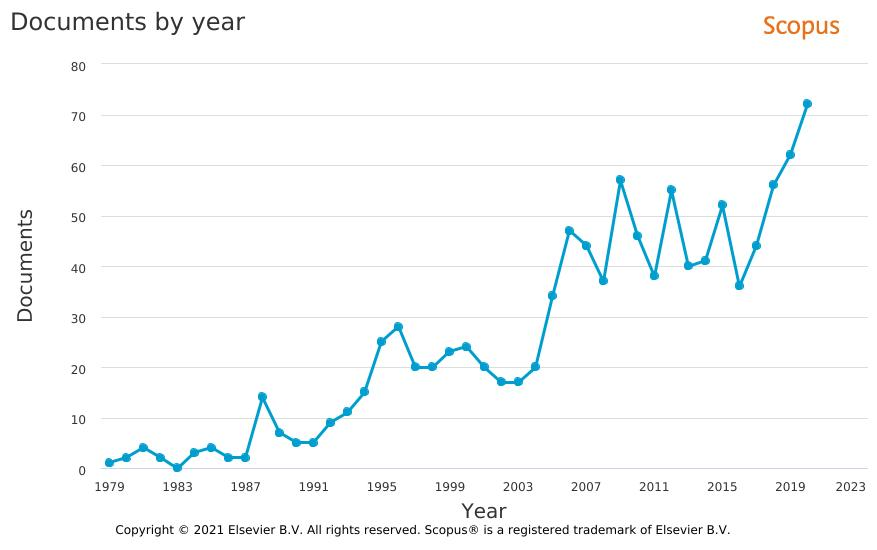
\includegraphics[width=0.49\textwidth]{Images/1979-2020.jpg}
  \caption{Cantidad de artículos por año. Scopus (Elsevier B.V, 2021).}
  \label{yearResults}
\end{figure}

Centrando un poco hacia el intervalo de tiempo trabajado en el presente artículo con el uso de la segunda ecuación de búsqueda, es posible apreciar que, de los 1067 documentos presentes en la base de datos de manera inicial, un total de 542 documentos fueron publicados entre 2010 y 2020. Es decir, alrededor del 51.08\% de los artículos publicados han sido de los últimos 10 años, demostrando así el creciente interés en el tema.

En cuanto a las áreas con mayor interés en la metodología de sistemas blandos se presenta, tras una búsqueda rápida en \textit{Scopus (Elsevier B.V, 2021)} que, como se puede apreciar en la figura \ref{subjectResults}, son las ciencias de la computación, con un 19.8\% de los artículos; negocios, gestión y contabilidad, nuevamente con un 19.8\% de los artículos; e ingeniería, con un 13.6\% de los artículos; como las 3 principales áreas en las que la MSB es aplicada o usada.

\begin{figure}
  \centering
      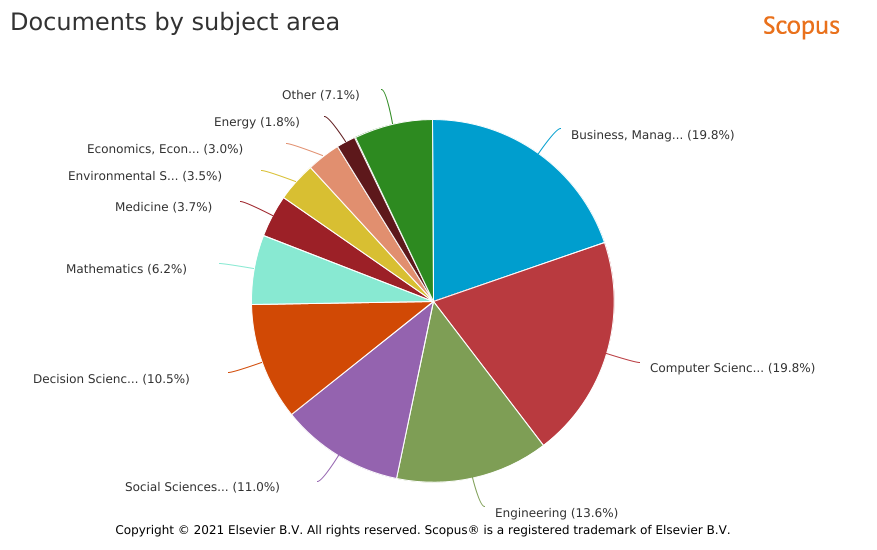
\includegraphics[width=0.49\textwidth]{Images/subjects.png}
  \caption{Repartición de artículos por área. Scopus (Elsevier B.V, 2021).}
  \label{subjectResults}
\end{figure}

\subsection{Modelados Conceptuales}
En términos generales, lo que se conoce de manera general como \textit{modelos conceptuales}, es un principal acercamiento a la formación de diferentes representaciones de los diferentes sistemas, subsistemas, al igual que los procesos desarrollados dentro de la organización. De igual manera, es necesario nombrar que estos modelos conceptuales, tienen cierto grado de abstracción que depende de las necesidades identificadas durante el desarrollo de lo requerimientos problema a resolver \cite{Adgeo[1]}. En este sentido, es de gran importancia que el desarrollo de estos modelos, cumplan verdaderamente su función y realicen un buen paralelo con la realidad puesto que es a base de esto en lo que se desarrollan las actividades de desarrollo e implementación que, en el caso de ser erróneas debido a un mal modelado conceptual, sería una directa pérdida de tiempo y dinero \cite{Pereira[1]}.

Entonces, debido a las funciones que los modelados conceptuales cumplen, una de las ramas de interés en las cuales se ha aplicado de manera directa ha sido la metodología de sistemas blandos con el fin de servir tanto de medio guía como un apoyo directo en la formulación de estos modelos conceptuales de las diferentes organizaciones. Esto se debe a que, como fue anteriormente descrito, la MSB, tiene la capacidad de identificar las diferentes partes del sistema al igual que los distintos componentes sociales los cuales son considerados relevantes para la búsqueda de la solución del problema. \cite{Checkland[2]}

Para el año $2011$, ya se estaban realizando aplicaciones de la metodología de sistemas blandos en los campos de desarrollo de modelos conceptuales. Uno de estos ejemplos se refiere al desarrollo de un modelo conceptual para el manejo de los recursos tanto eléctricos como utilidades dentro de una procesadora de textiles. En este caso, Ngia \textit{et al.}, se aplicaron los conceptos relacionados con el \textit{CATWOE} al igual que las \textit{Rich Images} de Peter Checkland para identificar los objetivos de la organización al igual que los clientes y las partes importantes de la misma. En este sentido, la aplicación de la metodología de sistemas blandos está presente con el fin de realizar un análisis de las actividades y actores que permiten el desarrollo de los procesos de las actividades económicas. Es decir, gracias a los conceptos identificados a partir de la aplicación de algunas de las partes de la metodología de sistemas blandos, se posibilitó el modelado al igual que la compresión de la procesadora de textiles. A partir de esto, se permitió el desarrollo de los requerimientos funcionales como no funcionales para los sistemas EUMSS (\textit{European Union Maritime Security Strategy}) que permitirían la mejora en el manejo de los diferentes recursos requeridos para el desarrollo de las actividades de la procesadora de textiles. \cite{Ngai[1]}

De igual manera, para el año $2014$, Pereira \textit{et al.}, vieron las posibles aplicaciones que tendría la metodología de sistemas blandos como una herramienta para el desarrollo de los diferentes modelados conceptuales que eran necesarios para el desarrollo de simulaciones de eventos discretos. Gracias a la capacidad de la MSB de trabajar como un \say{acercamiento a la solución de problemas complejos} \cite{Pereira[1]}. En este caso, aunque bastante similar al presentado por Ngai \textit{et al.}, se define con mayor claridad la relación entre el modelado y la aplicación de la MSB para la realización de la misma. La aplicación de las herramientas de la metodología se basaban principalmente para el modelado de las actividades de gran importancia. La aplicación de \textit{CATWOE} para la identificación de los objetivos principales al igual que el desarrollo de figuras que permitían el entendimiento del desarrollo de simulaciones de eventos discretos \cite{Pereira[1]}.

De esto, podemos ver la útilidad que presentan las herramientas desarrolladas por Peter Checkland en la formulación de modelos pertinentes de las diferentes problemáticas a trabajar. Al igual que la relativa prominencia que la metodología de sistemas blandos aún posee dentro de las diferentes áreas en la última década.

\subsection{Desarrollo Sostenible}
Debido a la gran importancia e interés que ha tenido el desarrollo sostenible en pro de la búsqueda de un mejor manejo de los recursos ambientales presentes, una de las áreas en las cuales la metodología de sistemas blando ha tenido un gran impácto ha sido dentro de la solución de problemas con ámbitos tanto ambientales como sociales en búsqueda de un mejor desarrollo ambiental.

Una de las maneras en las que se realiza este acercamiento por parte de la metodología de sistemas blandos hacia la problemáticas holistas del desarrollo sostenible está dado por el análisis realizado a las diferentes ramas relacionadas con el desarrollo ambiental. En este sentido, Sridan \textit{et al.} desarrollaron una aplicación de la MSB hacia todas las ramas relacionadas con el desarrollo ambiental en Tailandia. En este estudio, se realizan varios estudios relacionados con la disponibilidad de las materias primas, el manejo tecnológico y ambiental al igual que las políticas y leyes relacionadas con el ambiente. En este sentido, estas distinciones realizadas son las que permiten entender la problemática así como el desarrollo de los diferentes modelos de las actividades que cada una de las ramas analizadas realiza. Es así el como la aplicación de la metodología permitió la identificación de las diferentes acciones y medidas a tomar con el fin de dar una mejor a las problemáticas ambientales en las cuales debe actuarse \cite{Sridan[1]}. En este sentido, es posible observar el alto impacto que puede tener la metodología de sistemas blandos en los problemas de casi cualquier área en la cual esta pueda ser aplicada. 

En términos más locales, la aplicación de la metodología de sistemas blandos también hace parte de estudios dentro del país en términos de desarrollo ambientales. En términos generales, la aplicación de los sistemas blandos dentro de la ejecución de los diferentes frentes a trabajar eran los mismos que en el caso anterior. Sin embargo, la principal característica a resaltar del trabajo realizado por Acero \textit{et al.} recae en las personas que hicieron parte del desarrollo de la metodología, no hacían parte directa de las instituciones responsables, sino que eran parte de la comunidad, específicamente estudiantes, directamente afectada por los diferentes problemas ambientales de la zona trabajada \cite{Acero[2]}. En este sentido, es posible apreciar al alcance que tiene la metodología en cuanto esta puede ser aplicada a los diferentes actores dentro de la problemática con el fin de dar cabida a los diferentes componentes de una misma problemática. En cuanto al desarrollo de la problemática, la metodología de sistemas blandos permitió el desarrollo de diferentes soluciones años después a partir de los modelos desarrollados de manera inicial por los integrantes de la comunidad con el fin de dar solución a las distintas raíces identificadas \cite{Acero[1]}.

\subsection{Desarrollo de Software}
Con el aumento de la complejidad de las tecnologías con el paso de los años, los procesos de desarrollo cada vez han requerido de un aumento tanto en la cantidad de mano de obra como en el tamaño de las estructuras que componen las aplicaciones contemporáneas. En este sentido, uno de los enfoques en los cuales la metodología de sistemas blandos ha sido aplicada, recae la industrial relacionada con el desarrollo de software. Esto se debe a las capacidades, como se ha visto a lo largo del presente documento, que tiene la metodología de sistemas blandos a acercarse a los problema y desarrollarlos de manera holista. En este sentido, la MSB permite realizar estudios y distinciones sobre temas relacionados con implementación de estrategias de desarrollo e incluso, como era de esperarse, el levantamiento de requerimientos para el desarrollo de manera general.

Estas dos aplicaciones anteriormente nombradas hacen parte de algunas de las categorías en las que la MSB se ha destacado en la última década. Primeramente, la metodología de sistemas blandos fue empleada con el fin de evaluar y comprender el fallo de la implementación de la estratégia \textit{Agile} para el desarrollo de software para los \textit{early adopters} del framework. Para el caso de Suryaatmaja \textit{et al.}, es de destacar como tal el enfoque el cual estaba teniendo la metodología en comparación con los demás casos presentados, esto se debe a que, en comparación sobre una organización específica, la aplicación de la MSB estaba más enfocada a una cantidad general de problemáticas identificadas para varios grupos en los cuales, el framework de \textit{Agile} había fallado. En este sentido, la aplicación de tanto modelos conceptuales como el análisis de las raíces de la organización a partir de CATWOE, permitieron el entender los factores determinantes que debían ser identificados para entender de manera general las intenciones y las visiones de las diferentes organizaciones que fueron estudiadas de manera indirecta. Del mismo modo, la aplicación de las diversas herramientas pertenecientes a la metodología de sistemas blando, permitió la el identificar tanto los problemas como las posibles decisiones a tomar con el fin de dar solución al problema en cada uno de los aspectos identificados \cite{Suryaatmaja[1]}.

Análogamente, la determinación de los requerimientos para el desarrollo, como parte importante del desarrollo de cualquier tipo de proyecto no trivial de software, es una de las partes más importantes dentro de la fase de planeación en cuanto estas, de manera general, son empleados como la guía en cuanto a las necesidades a satisfacer con la solución de software planteada. Una aplicación de esta necesidad puede verse trabajada desde la perspectiva de la metodología de sistemas blandos dentro de la problemática general trabajada por Albareta \textit{et al.} en la cual, la intención de aplicación de la MSB está enfocada de manera principal como una herramienta para entender la situación a resolver. A búsqueda de cumplir este fin, la aplicación de las diferentes partes de la MSB, están dadas a "identificar una situación de la vida real que se considere problemática" y también "La situación problemática expresada en términos de \textit{Rich Images}". Todo esto, se da con el fin de identificar tanto los requerimientos como la posible manera de resolverla partiendo de la idea de los Procedimiento Operativo Estándar (SOP) \cite{Albareta[1]}. 

\section{Conclusiones}
Tras el desarrollo de las diferentes temáticas, en conjunto con la identificación de las aplicaciones de la metodología de sistemas blandos, nos permitieron comprender tanto el alcance como el impacto de estos acercamientos holistas a las diferentes problemáticas trabajadas durante la extensión del presente artículo. En este sentido, el entender el actual estado de la MSB como una herramienta más en las diferentes áreas de investigación, nos da a entender que, efectivamente, esta aún cumple su propósito de ser una forma de dar cabida al desarrollo de soluciones donde se entienden todos los aspectos de las organizaciones en los cuales esta es aplicada.

%bibliografía
\bibliographystyle{IEEEtran}
\bibliography{BiblioTexto}

\end{document}
